\section{Dataset And Feature Extraction}
\label{sec:data}
In this section we discuss the properties of the dataset we use for our experiments as well as feature extraction techniques adopted.

\subsection{YouTube Dataset}
\label{sec:youtubedataset}
We apply classification techniques on a sample dataset taken from YouTube~\cite{youtubedata}. 
This dataset includes $691407$ comments for $200$ most trending YouTube videos in US in a two weeks period. 
The same source also offers a similar dataset for the most trending videos in GB. 
We will use a fraction of this dataset as our test set for sentiment analysis. 
The data includes comment data and video data. The comment data maps video IDs to comments and the number of likes and dislikes for the corresponding comments. The video data contains video title, channel title, category, tags, number of views, likes and dislikes and user reviews. The US videos belong to $15$ categories.

\begin{figure}%
\centering
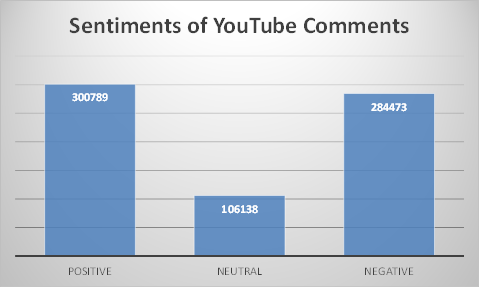
\includegraphics[width=1.0\columnwidth]{figures/datastats.png}%
\caption{YouTube Dataset Statistics}%
\label{fig:datastats}%
\end{figure}

\subsection{Label Generation}
\label{sec:label}
Our goal is to classify YouTube comments into positive, negative or neutral sentiment classes. However, there are no labels showing the sentiment of the comments. Considering the large number of comments, it was not possible for us to manually label a reasonable fraction of this dataset. Consequently, we used the TextBlob~\cite{textblob} library for Python to generate the labels. TextBlob applies NLP (Natural Language Processing) techniques to estimate the \textbf{polarity} of each comment independently from the rest of the comments, and only based on its content. For us, it replaces the burdensome task of manual labeling. TextBlob generates polarity scores in the range of $(-1,1)$. We convert them into categorical data using the following equation.
\begin{eqnarray*}
\textrm{sentiment}=
\begin{cases}
-1 & \textrm{polarity} < 0\\
0 & \textrm{polarity} = 0\\
1 & \textrm{polarity} > 0
\end{cases}.
\label{eq:sentiment}
\end{eqnarray*}
Statistics on the population of each class is shown in Figure~\ref{fig:datastats}.
Words that happen more frequently in positive and negative comments are shown as word clouds in Figures~\ref{fig:poscloud} and~\ref{fig:negcloud}.
In Section~\ref{sec:cat-exp}, we do category classification based on tags and comments. The category labels are already available in video data.

\begin{figure*}[tb]%
\centering
\begin{tabular}{cc}
\subfloat[Word cloud for positive comments \label{fig:poscloud}]{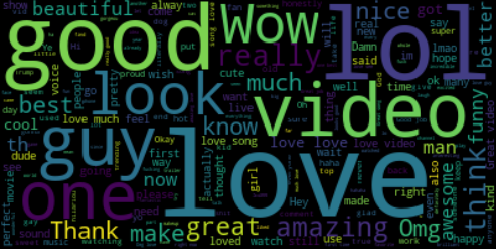
\includegraphics[width=0.95\columnwidth]{figures/pos_WordCloud.png}} & 
\subfloat[Word cloud for negative comments \label{fig:negcloud}]{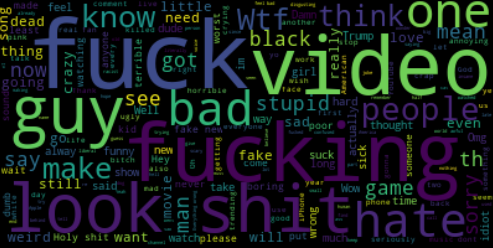
\includegraphics[width=0.95\columnwidth]{figures/neg_WordCloud.png}}
\end{tabular}
\caption{Word cloud of common words in YouTube comments}
\label{fig:wordcloud}
\end{figure*}


\subsection{Feature Extraction}
\label{sec:feature}
For sentiment classification based on comments, we used TF-IDF~\cite{massiveDatasets} to convert comments into feature vectors. In this technique, TF (Term Frequency) counts the number of times a word has occurred in each document. However, the number of occurrences of words is in general higher for longer documents. Then, it is helpful to divide the number of word occurrences by the number of words in the document. The output of TF is a sparse matrix mapping documents to a normalized vector representing how many times each word has occurred in them. IDF (Inverse Document Frequency) accounts for the number of occurrences of a word in the entire document corpus. Namely, some words are more likely than others to happen in a given corpus of documents. Then, we scale TF terms by a decreasing function of the number of occurrences of each word in the whole corpus which is indeed the IDF term.

For category classification, we took two approaches. First, we used the same TF-IDF comment features. Second, we used the tags from the video data. Since video data has been gathered daily over two weeks, it may contain each video multiple times along with different tags. To remove duplicate entries, we removed punctuations and English stop words from the tags. Stop words are first removed. Stop words are commonly used words such as \textit{the} which are filtered out before the analysis. Then, the videos were grouped based on their ID and tags were aggregated taking their union. We denote the tags of a video by a binary feature vector where each entry is zero in case the video was tagged by the corresponding tag and zero otherwise.